\chapter{Background: Network Access Control}
Network Access Control (NAC) is the use of authentication protocols in combination with control policies to limit unauthorised access to network resources. \cite{cisco_why_nac}

A common use of NAC is Wi-Fi Protected Access (WPA), the security standard used to safeguard household wireless networks from unauthorised access. The personal version of WPA is achieved through the distribution of pre-shared keys (PSK). A PSK is a key that is distributed to all authorised users and is used during the authentication process to prove authorisation. It is also used to derive the symmetric encryption keys used for communication between the client and the wireless AP.

The PSK model is not a valid option for enterprise\cite{juniper_psk}, due to overhead on the event of staff turnover. If staff turnover occurs a new PSK must be generated and distributed to all remaining staff to fully remove the ex-employee's access. 

The PSK model also provides no accountability. As all clients share the same credentials there is no way to associate performed actions and traffic to specific authorised users on the network. Access logs can be creating using MAC addresses of devices but this is not viable solution as there is no clear association between devices and authorised users. Also authorised users could use disposable devices or spoof MAC addresses to perform malicious activities without revealing their identity.

To address these issues, the the Internet Engineering Task Force (IETF)\cite{ietf} proposed the Extensible Authentication Protocol (EAP)\cite{rfc_3748}. EAP is a framework by which authentication protocols can be written and provides common functions such as negotiation of EAP-methods.

An EAP-method is an individual authentication method. It defines the specifics of how authentication is to be performed between a user and server, but is not a line-protocol and does not provide a mechanism for transporting the messages across a network. There are over 30 EAP-methods defined with EAP-MD5, EAP-TLS, EAP-TTLS and EAP-PEAP being the most common.

All EAP-methods support individual authentication credentials for clients providing a solution for accountability, but does not define a mechanism for logging or authorisation management.

As EAP-methods do not define a line-protocol, an encapsulation layer must be used to transport EAP messages over a network. This encapsulation layer can be an Authentication, Authorization and Accounting (AAA)\cite{aruba_aaa} protocol allowing for additional attributes to be transported with EAP messages. These attributes can be used by network components to enforce authorisation policies and the supporting AAA servers can be used for storage of access request logs and user credentials.

\begin{figure}\begin{center}
    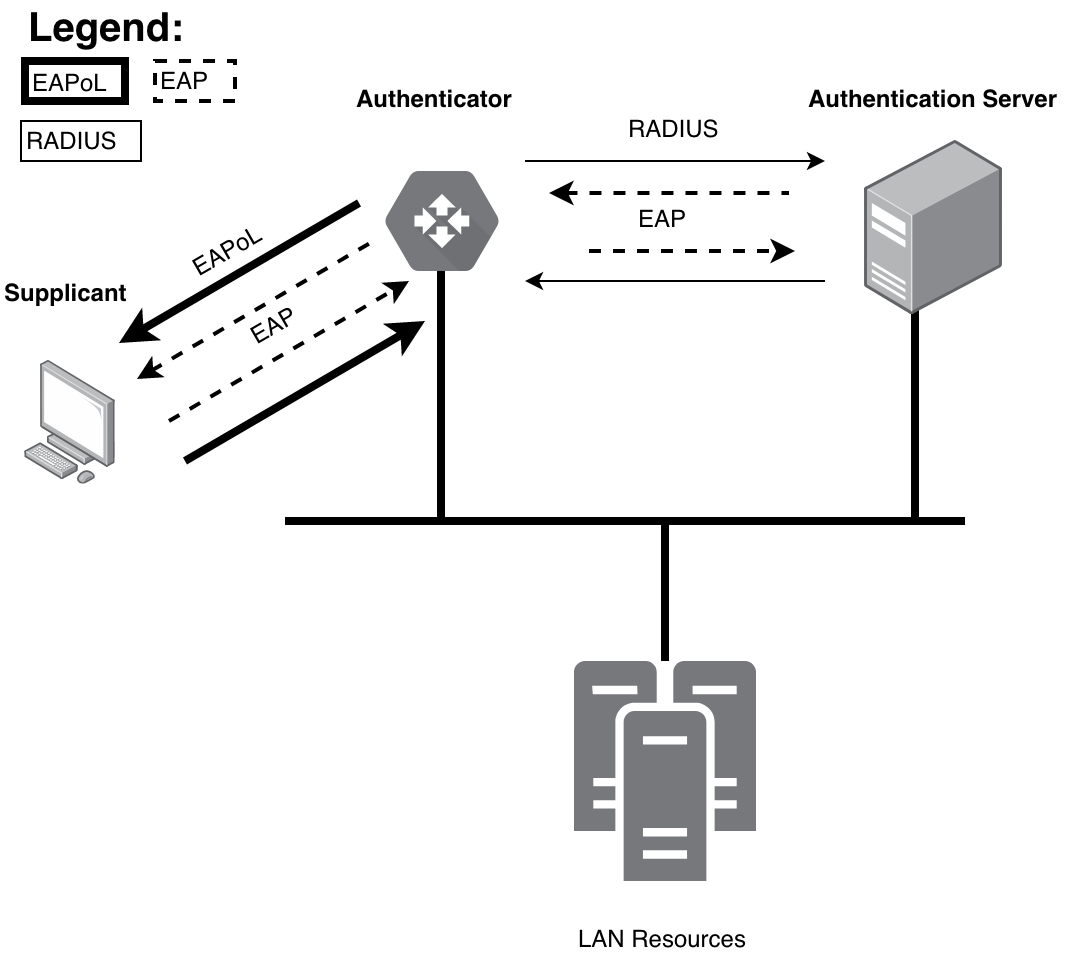
\includegraphics[height=6cm]{images/dot1x_wired_protocol.png}
    \caption{802.1x Protocol}
    \label{fig:802_wired_protocol}
\end{center}\end{figure}

The 802.1x protocol defines a port-based network access control solution for IEEE 802 networks. By creating a separation of authentication and access control, EAP-methods are used to perform authentication while 802.1x provides mechanisms for blocking ports. As EAP messages must be encapsulated, Ethernet headers are used to transport them over the LAN network. Before successful authentication is achieved all traffic, except required EAP messages, is dropped on a port. On successful completion of the EAP authentication process the port is opened and traffic is not dropped from the authenticated client.

\section{Extensible Authentication Protocol (EAP)}
EAP defines a framework for the design and development of network authentication protocols. It provides common functions and negotiation for authentication methods, these methods are known as EAP-methods. 

EAP-methods define the method used to provide identity verification throughout the authentication process. An example of an EAP-method is EAP-TLS. 

EAP is not a line-protocol and required an encapsulation protocol layer to send requests over a network. Examples of encapsulating protocols are EAPoL or RADIUS, which are discussed in further detail below.

The EAP framework splits the responsibilities of authentication into three main components. 
\begin{itemize}
    \item The Supplicant
    \item The Authenticator
    \item The Authentication Server
\end{itemize}
These components are expected in all EAP-methods and are required by protocols using EAP as the authentication method. The components are described in more detail below.

\subsection{Supplicant}
The Supplicant, also known as the peer in RFC 3784\cite{rfc_3748}, represents a client that wishes to join the controlled network. It communicates directly with the Authenticator, negotiating a supported EAP-method and provides credentials or authentication tokens to perform authentication.

\subsection{Authenticator}
The Authenticator receives EAP authentication requests from one, or many, Supplicants and forwards them to the Authentication Server. Is is responsible separating the Supplicant from the Authentication Server and provides a distributed network of authentication points. 

The Authenticator is used as the 'gate-keeper' of the network and is capable of performing authentication without the use of the Authentication Server.

\subsection{Authentication Server}
The Authentication Server is the primary store of client identities. It receives requests from one, or many Authenticator nodes and is generally used for performing EAP authentication with the Supplicant. [Refer to figure \ref{fig:802_packets}]

\begin{figure}\begin{center}
    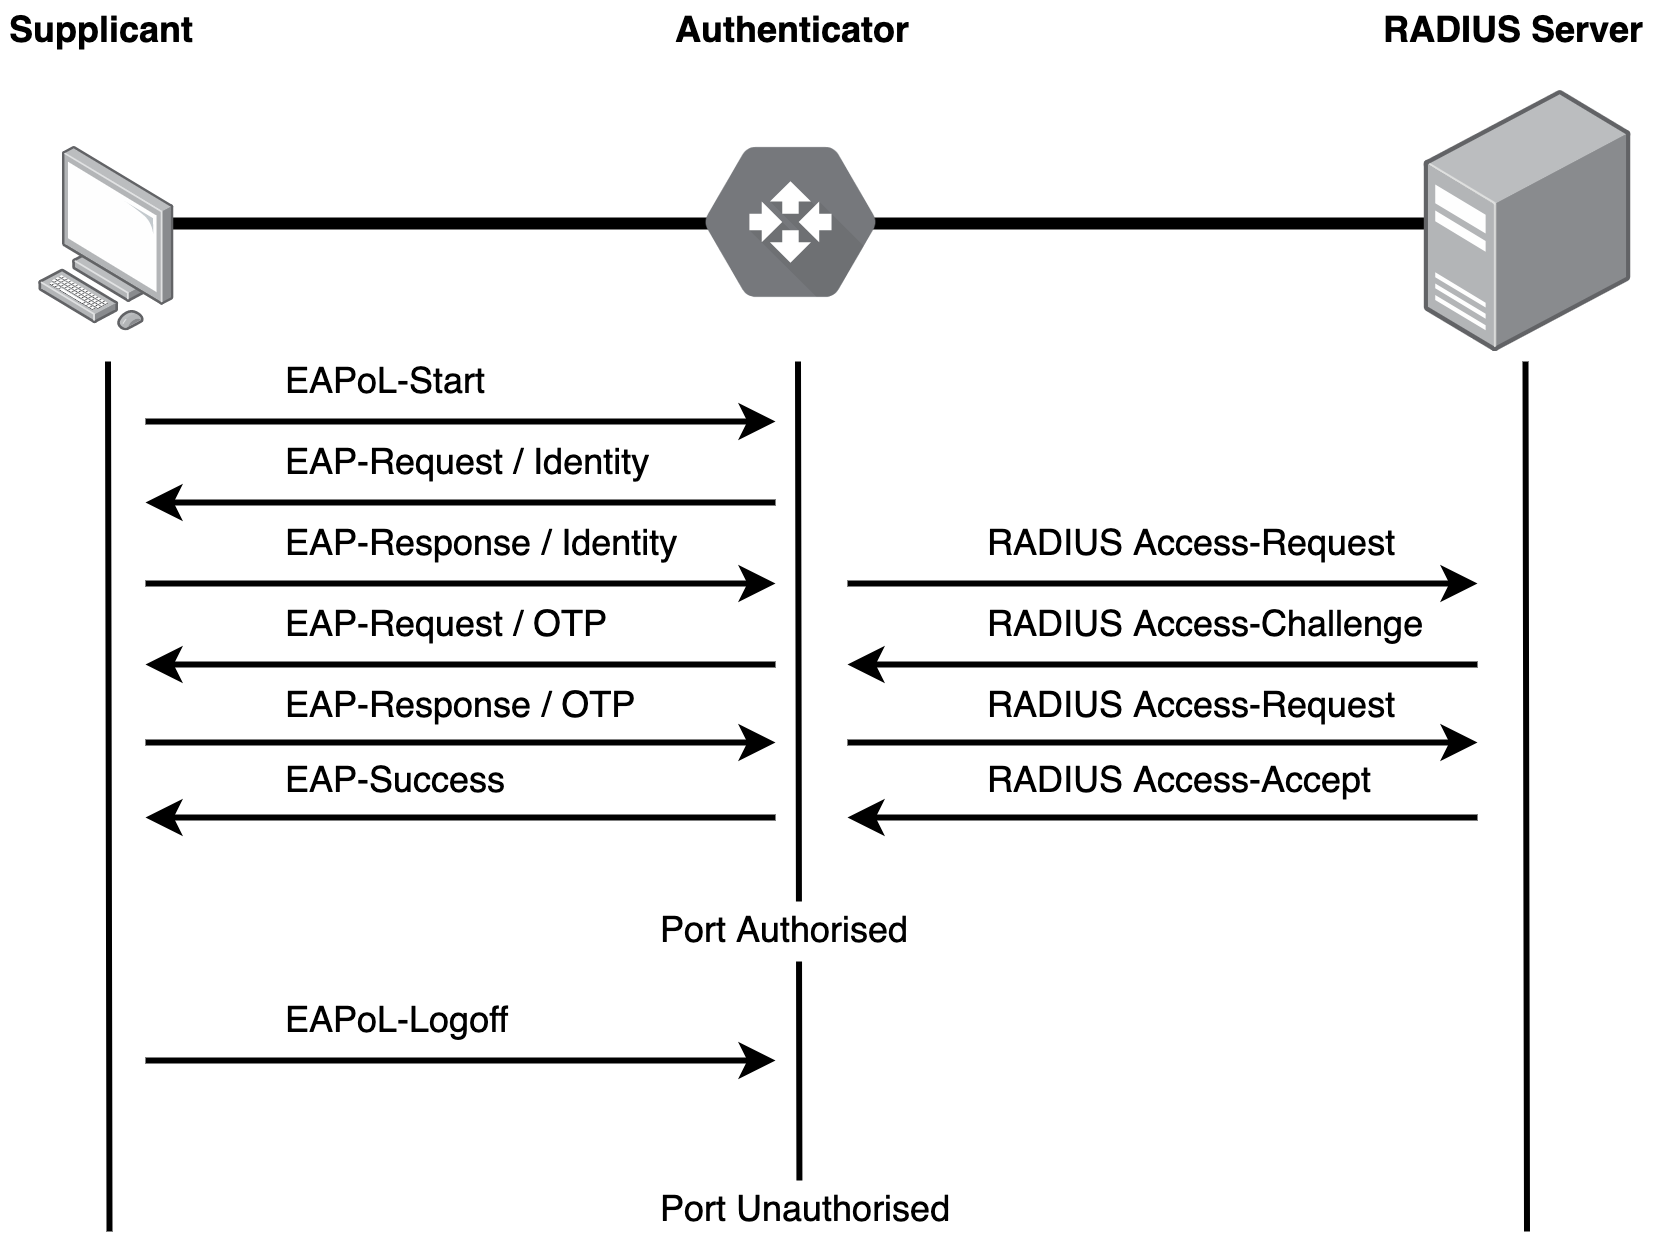
\includegraphics[height=6cm]{images/dot1x_packet_diagram.png}
    \caption{802.1x Packet Diagram}
    \label{fig:802_packets}
\end{center}\end{figure}

The Authenticator is also notified of completed authentication attempts by the Authentication Server. If the Authentication Sever is communicating using an AAA protocol at the encapsulation layer, it may provide access control policies to the Authenticator to be added as restrictions on the session that is created.

\section{Remote Authentication Dial-In User Service (RADIUS)}\label{sec:radius_packets}
Remote Authentication Dial-In User Service (RADIUS) is an AAA protocol. It can be used as an encapsulation protocol for EAP-methods and provides mechanisms for sharing AAA information that may not be available with other EAP encapsulation methods, such as EAPoL. 
In the 802.1x design, RADIUS is used for communicating EAP messages between the Authenticator and Authentication Server and is used to provide authorisation information to the Authenticator.
RADIUS servers also perform as Authentication Servers, providing additional functionality such as storing a centralised storage of authentication credentials, authorisation rules, accounting logs and other AAA information that is associated with user credentials in its credential-store. \cite{rfc_2904}
RADIUS also provides support for authentication without EAP by receiving user credentials through RADIUS-Attributes and perform authentication using the provided information.

There are 4 primary RADIUS packet-types used during RAIDUS authentication; Access-Request, Access-Challenge, Access-Accept and Access-Reject.

\begin{itemize}
    \item Access-Request:
    Initiates the authentication process with the server. It is used to provide credential information to the server and respond to Access-Challenge requests.
    
    \item Access-Challenge:
    Requests further information about the client and their credentials. This can include performing encryption / decryption functions using their private key to prove identity and is used for EAP authentication.
    
    \item Access-Accept:
    The user has successfully authenticated with the network as is to be granted access to network resources. RADIUS attributes can be attached to this message to provide session restriction requirements to the Authenticator.
    
    \item Access-Reject:
    The user has been unsuccessful with the authentication attempt and must not be granted access to network resources.
\end{itemize}

Special RADIUS Attributes can be attached to RADIUS Access-Accept messages used to notify an Authenticator about restrictions that must be placed on an authenticated session.
There are a large number of RADIUS attributes used for access restriction policies supplied as open-standards and vendor-specific attributes. 

During this project I will only be looking at open standard attributes \cite{radius_attributes_iana} provided by the IETF and IANA in an attempt to provide a multi-vendor support. The IETF have also provided a set of usage guidelines available for best practices that I will attempt to comply with.\cite{rfc_3580}\\
I have defined the attributes that are of note for this project below:
\begin{itemize} [leftmargin=*]
    \item [] \textbf{Attribute 64 | Tunnel-Type:}\\
    This attribute indicates the type of tunnel that will be used for the Supplicant's session. This can be used in conjunction with to Tunnel-Private-Group-Id to specify a VLAN to be allocated for a session.
    
    \item [] \textbf{Attribute 81 | Tunnel-Private-Group-Id:}\\
    This attribute indicates the name or ID of a tunnel in which the Supplicant's session will be placed. When used in conjunction with RADIUS 64 attribute, it can be used to define a VLAN ID.
    
    \item [] \textbf{Attribute 11 | Filter-Id:}\\
    This attribute indicates the name of a filter that will be applied to the Supplicant's session.\cite{juniper_filter_id}

    \item [] \textbf{Attribute 92 | NAS-Filter-Rule:}\\
    This attribute indicates an individual filter rule that can be applied to the Supplicant's session. The format of the rule is not clearly defined in the specification however the two main approaches implemented by main vendors. 
    
    Cisco implements dACLs using a vendor-specific alternative that contains iOS terminal commands for setting up an ACL.\cite{cisco_filter_rule}. 
    
    HPE uses the standard attribute [91] and has attempted to standardise the format of a rule, defining both an allow and deny rule syntax. \cite{hpe_filter_rule}
\end{itemize}

Note, for most vendor implementations the Filter-ID and Tunnel-Private-Group-Id attributes should be used to identify existing resources and does not guarantee the creation of VLANs, ACLs or other filters.

\section{Extensible Authentication Protocol over LAN (EAPoL)}
Extensible Authentication Protocol over LAN (EAPoL) is a line-protocol for EAP messages. It is used to encapsulate and transport EAP messages over an IEEE 802 network.

EAPoL encapsulates EAP messages in Ethernet frames. This provides a generic solution for port-based authentication as Ethernet is supported protocol of traditional networking equipment. 
EAPoL frames can be identified by their ether-type of 0x888e and support transport of all EAP-methods as encapsulation of the whole EAP message is achieved. [Refer to Figure \ref{fig:EAP_layers}] 

\subsection{The Authentication Process}
When a Supplicant connects to a controlled port, it sends an EAPoL-Start message to the multi-cast address 01:80:c2:00:00:03. Authenticators controlling the network boundaries receive these requests and initiate the authentication process. [Refer to Figure \ref{fig:802_packets}]

The authentication process consists of the 5 steps discussed below:
\begin{enumerate}
    \item On receiving the EAPoL-Start message, the Authenticator sends an Identity-Request in response to the Supplicant requesting further credential information.
    
    \item The required credential information is packaged into an EAP Identity Response and forwarded through the Authenticator to the Authentication Server.

    \item On the Authentication Server receiving the Identity-Response a challenge is generated and provided back to the Supplicant.

    \item The Supplicant completes the requested challenge using the EAP-Method that is relevant, and an EAP-Request is sent back to the Authenticator for processing by the Authentication Server.

    \item On successful authentication, the Authenticator will receive the EAP-Success message and open the port. On an unsuccessful authentication attempt, the Authenticator will receive the EAP failure message and the port will remain closed. 
    
\end{enumerate}

\begin{figure}\begin{center}
    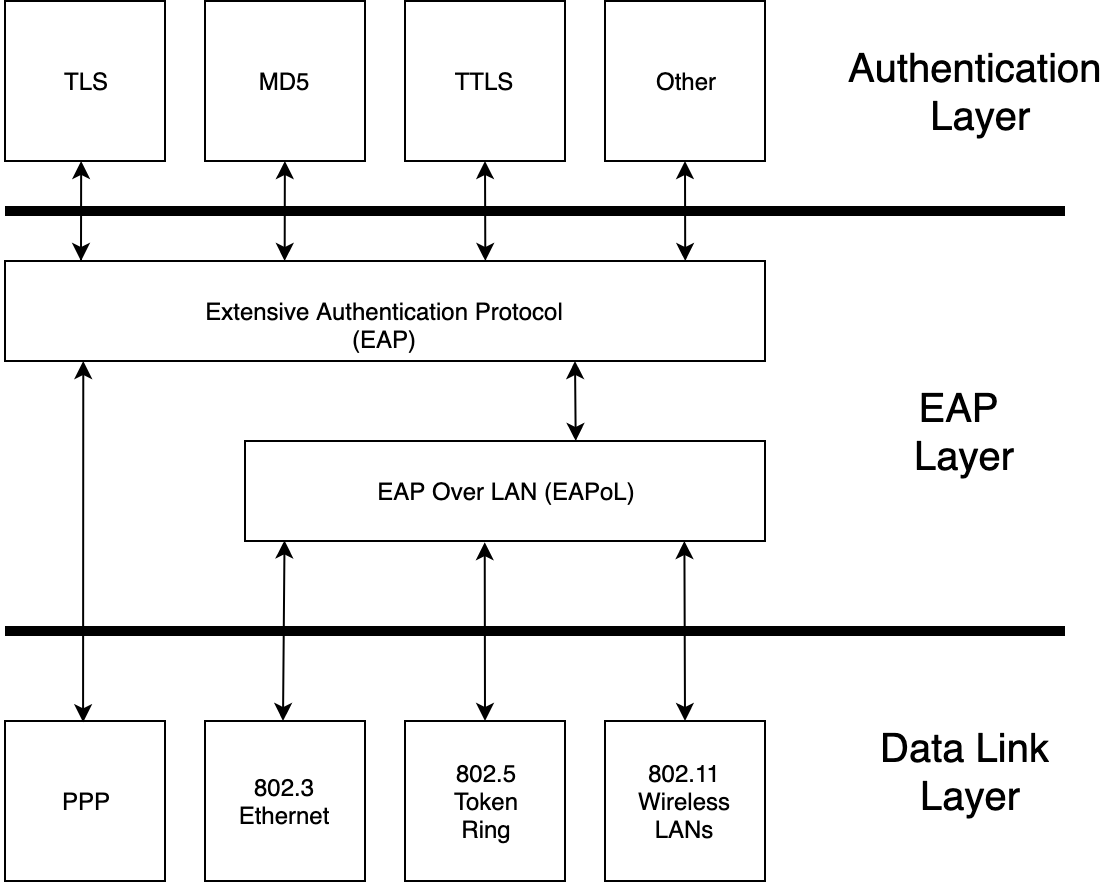
\includegraphics[height=6cm]{images/eap_layers_diagram.png}
    \caption{EAP Layers}
    \label{fig:EAP_layers}
\end{center}\end{figure}

\section{IEEE 802.1x Protocol}
The 802.1x protocol defines a port-based network access control solution by combining the use of EAPoL and RADIUS.

A separation of authentication and access control is created by using EAP-methods to perform authentication and RADIUS messages to transport AAA-related information.

Communication between the Supplicant and Authenticator is achieved using EAPoL to transport EAP messages over the Ethernet network. Communication between the Authenticator and the Authentication Server; referred to as the RADIUS server; is achieved using RADIUS to transport EAP messages.

All traffic, excluding EAPoL traffic, is dropped by the Authenticator; Blocking unauthenticated clients from accessing networking resources and requiring a successful authentication attempt before the port is opened for network access.

On completion of a successful authentication attempt, the Authentication Server will provide the Authenticator with any access restrictions defined in its credential-store as RADIUS attributes. These attributes can be used by capable Authenticators to apply VLANs or ACLs on client sessions before opening controlled ports. [Refer to Figure: \ref{fig:802_wired_protocol}]

Capabilities of filtering on a controlled port include; limiting the type of traffic that users can send, limiting access to resources and placing users on separate VLANs. A practical example of this could involve actions such as filtering all RDP traffic for all non-technical staff or placing all members of a work-team in the same VLAN.

As 802.1x provides a NAC solution for IEEE 802 networks it can be paired with WPA to provide an enterprise alternative to the PSK implementation. When clients connect, their authentication requests use individual credentials and all other traffic is blocked until successful authentication is achieved. This removes the overhead of WPA-PSK on the event of staff turnover and provides the ability for logging individual network access requests.

\section{MAC Authentication Bypass}
MAC Authentication Bypass (MAB) is a method of providing access to an 802.1x controlled network for devices that are unable to perform EAP authentication. MAB performs a MAC-based authentication attempt on behalf of a connecting client. This authentication then occurs without the knowledge of the client, and access is granted on a successful authentication attempt.

A MAB-enabled Authenticator is notified of a connecting client through Dynamic Host Configuration Protocol (DHCP) broadcast requests. The DHCP broadcast messages are sent by new clients requesting configuration information of the local network. This allows clients to configure themselves in accordance with the network policies. 

From these requests the Authenticator can extract the source MAC address, build an AAA Access-Request containing the MAC information and send this to the Authentication Server. 

As the authentication is performed between the Authenticator and Authentication Server, AAA authentication methods can be used and EAP-methods are not required. The MAC address information can be provided to the Authentication server using AAA attributes and the authentication can be performed without a challenge being performed by the Supplicant.

As MAB uses MAC addresses for authentication\cite{cisco_mab} it is a less secure alternative to EAP and should only be applied on an individual port basis. NIC drivers can be used to obfuscate their original MAC with a user-defined MAC. This is known as MAC address spoofing and can be used to authenticate to a MAC-based authentication system. However, this is more secure than leaving open ports for devices that are unable to perform EAP-based authentication.